%%%%%%%%%%%%%%%%%%%%%%%%%%%%%%%%%%%%%%%%%%%%%%%%%%%%%%%%%%%%%%%%%%%%%%%%%%%%%%%
\section{Aberration Measurement and Correction}
\label{Measurement}
%%%%%%%%%%%%%%%%%%%%%%%%%%%%%%%%%%%%%%%%%%%%%%%%%%%%%%%%%%%%%%%%%%%%%%%%%%%%%%%


In practice, no optical system can be totally free from aberrations. That means that all the rays originating from the same object point and going through an optical system will not converge into the same point at the image plane. In other words, the wavefront is distorted with respect to an ideal one when passing through a real system. Thus, we can define the wavefront aberration function as the optical path difference between the aberrated~(real) wavefront and the reference~(perfect) wavefront. These aberrations can be introduced both upon reflection from a non-planar irregular surface and by passing through an inhomogeneous media as shown in Fig.~\ref{fig:abberations}. 

\begin{figure}[tbh]
       \centering
        \begin{subfigure}[b]{0.4\textwidth}
                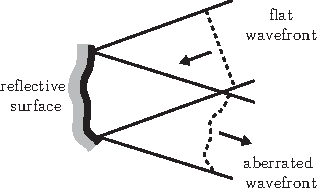
\includegraphics[width=\textwidth]{images/wavefront_distortions_reflection}
                \caption{Reflection.}
                \label{fig:abberation_reflection}
        \end{subfigure}
				\hspace{1em}
        \begin{subfigure}[b]{0.3\textwidth}
                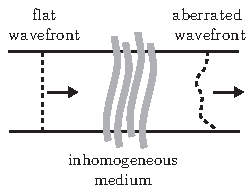
\includegraphics[width=\textwidth]{images/wavefront_distortions_transmission}
                \caption{Transmission.}
                \label{fig:abberation_trans}
        \end{subfigure}
        \caption{Wavefront aberrations due to (a) reflection from a non-planar surface and (b)  caused by propagation through a non-uniform 
refractive index distribution~\cite{AOM_basic_ref}.}
\label{fig:abberations}
\end{figure} 

In biological microscopy, the two potential sources of aberrations are the optics and the specimen under study. Regarding the optics, one important parameter is the Numerical Aperture~(NA), a higher NA not only increase theoretically the resolution but also aberrations become more significant. Besides, aberrations might also come by the difference of refractive index between the microscope coverslip and the specimen mounting medium. Regarding the specimen, aberrations are mainly caused by the variations in refractive index due to the three-dimensional nature of cells and tissue structures. These sample induced aberrations generally become dominant when the image focus lies deep within the sample, since light hast to pass a large distant trough an inhomogeneous medium~\cite{AOM_basic_ref}. 

There are different ways to characterize the aberrations mathematically. In systems with circular symmetry~(circular apertures) it is very common to use the Zernike polynomials because they form a complete, orthogonal set of functions defined over a unit circle~\cite{Zernike_original}:
\begin{align}
	\ W(\rho,\phi) = {\sum_{n}^{k}}{\sum_{m=-n}^{m=n}}{{c_n}^m {Z_n}^m}{(\rho,\phi)},
	\label{eq:aberration_zernike}
\end{align}
where $W(\rho,\phi)$ is the wavefront aberration function in polar coordinates at the exit pupil, $c_n^m$ are the Zernike coefficients and $Z_n^m (\rho,\phi)$ are the Zernike modes~(or polynomials). As we can see in the equation, the wavefront aberration function is a linear combination of polynomials. Therefore, the more polynomials~(i.e. modes, $Z_n^m (\rho,\phi)$) we can measure, the better characterization of the $W(\rho,\phi)$ function we have.
Representing aberrations in this way can simplify the design, control and characterization of the Adaptive Optics system specially due to the independence of each polynomial with respect the others. This powerful property is given by the orthogonality. 

Although it is known where the aberrations come from, it is not always easy to measure them and implement the measure inside the optical system. There are different classifications of wavefront sensing in the bibliography~\cite{AO_engineering_handbook}. Here we will use the one employed by \emph{Martin J. Booth}~\cite{AOM_basic_ref} and we will explain the most common methods of wavefront sensing applied to microscopy.     
     
%%%%%%%%%%%%%%%%%%%%%%%%%%%%%%%%%%%%%%%%%%%%%%%%%%%%%%%%%%%%%%%%%%%%%%%%%%%%%%%
\subsection{Direct Wavefront Sensing}
\label{sec:WavefrontSensing}

Direct Wavefront Sensing is based on a direct measure of the phase gradient or the wavefront slope, it is considered as an aperture-plane sensing. Within this group there are several techniques such as interferometric, although in general the most used is the Shack-Hartmann. 

The Shack-Hartmann technique is based on a two-dimensional array of lenslets -a matrix of microlenses- all with the same diameter and the same focal length. When an incoming beam goes through the matrix gets split and multiple focal spots are recorded onto the detector, which is placed at the focal plane of the microlenses, as shown in Fig.\ref{fig:SH}. The recording device is usually a CCD camera and typical microlens diameter range from about 100 to $\unit[600]{mm}$ with typical focal lengths ranging from a few millimeters to about $\unit[30]{mm}$~\cite{AO_vision_science}. By measuring the displacements with respect the optical axis~($\Delta x, \Delta y$) of each focal spot~(Fig.~\ref{fig:SH}) it is possible to reconstruct the wavefront slopes and finally to obtain the wavefront aberration function. It is important to take into account that this technique loses its accuracy for strong aberrated wavefronts, mainly due to overlapping of focal spots or crossover.

\begin{figure}[htbp]
	\centering
		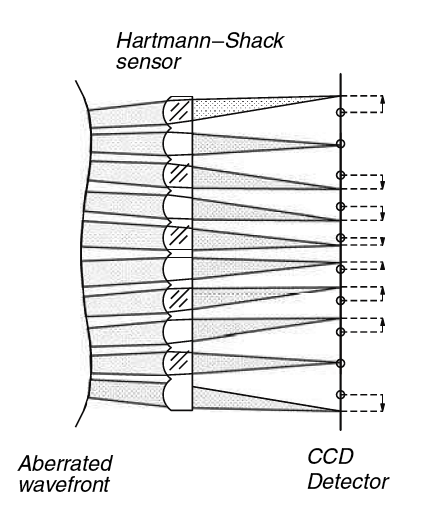
\includegraphics[width=0.30\textwidth]{images/SH}
	\caption{Two-dimensional section of Shack-Hartmann matrix of microlenses. An incoming beam is divided and imaged onto a CCD~detector. This generates separate focal spots for each microlens. If the wavefront is not aberrated, each spot will be placed along the central axis of each microlens. If it is aberrated, it will be displaced with respect to this axis and a wavefront reconstruction can be performed based on the magnitude and direction if this displacement. Image after~\cite{optical_shop_testing}.}
	\label{fig:SH}
\end{figure}

While the basic idea of this sensing techniques is simple, we must note that a well defined wavefront in the pupil of the system is required, which can only be produced by a point-like emitter. When studying three-dimensional, biological specimens, a single point-like emitter is usually not encountered which leads to a number of problems. The first one is the superposition of wavefronts coming from the light in the focal region and the light out-of-focus. These superposition depends on the coherence of the emitted light. Coherent light will cause interference in the pupil, thus causing ambiguous sensor readings rendering the measurement useless for aberration correction. Also, another problem that can arise is that the sensor might detect more signal intensity from the light out-of-focus rather than the light from the focal region. In order to overcome this situation, a spatial filter between objective and sensor can be used, much like the pinhole used in confocal microscopy. It is also possible to use coherence gating to exclude out-of-focus light instead of the spatial filter, although it is a more complex method~\cite{scan_TPFM_gated_wavefront}. 

However, if the specimen behaves as a point-like emitter, it still needs some restrictions in order to apply direct sensing. That is because if coherence light is used and the specimen has a planar-mirror behavior in the focal region, the sensor will just be able to measure twice the even components of the aberrations produced in the illumination path~(or emission path). This is due to the spatial inversion caused by any mirror and the interference between the illumination and emission wavefronts, as shown in Fig.~\ref{fig:abe_direct_sensing}). Hence we lose information about aberrations and indirect sensing schemes should be preferred. But if the specimen behaves as a point-like scatterer, it will emit incoherent light and the sensor will measure the aberrations produced in the emission path. In this case direct sensing can be applied.  

\begin{figure}[htbp]
	\centering
		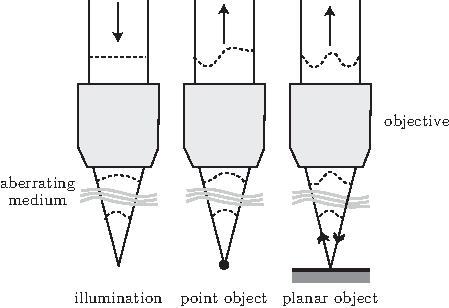
\includegraphics[width=0.50\textwidth]{images/abe_direct_sensing}
	\caption{Representation of the two effects due to the specimen structure on wavefront measurements. The left figure shows how the wavefront is aberrated in the illumination path. In the center it is shown a point-like scatterer. Only the emission path is measured. In the right figure it is shown a planar reflector. The illumination wavefront is spatially inverted on reflection before acquiring further aberration in the emission path. Image after~\cite{AOM_basic_ref}.}
	\label{fig:abe_direct_sensing}
\end{figure}

Nowadays, the most common approaches of direct sensing to microscopy are the use of Two Photon Excitation Fluorescence (TPEF) technique or the use of fluorescence microspheres. In the first one, microscopists take advantage of not only the incoherent emission due to the fluorescence process but also of the light confined in the focal region due to the nonlinear process. Therefore, a point emission is present and it is possible to apply direct sensing. More details can be found in section~\ref{sec:TPFMDirect}. Another approach is to create a point-like scatterer, a fluorescenct microsphere, and insert it into the sample. These microspheres are treated beads capable of emitting in different colors such as blue, crimson, red, orange, green or yellow, resistant to different conditions and with diameters that more or less go from 0.01 to $\unit[4]{\mu m}$. They can be engineered to target different biological tissues and there are several ways to insert these microspheres into the sample such as negative pressure injection, pressure injection, matrotrophycally or diffusion. Since they are loaded with fluorescent dyes, an excitation beam is needed to activate the fluorescent emission. This may be taken into account if direct sensing is applied to fluorescence microscopy. In this case, two excitation beams and two detection devices need to be used. One beam is needed  for the wavefront sensing, linked with the fluorescence of the microsphere, and one for imaging the sample. Another important characteristic about this method is related with the microsphere density and localization. Once the beads are inserted into the sample it is not possible to control their distribution or positions, thus, a certain density of microspheres is necessary in order to cover enough sample for sensing. Although it is an invasive method and seems to add more complexity to the system, \emph{Azucena et al.} showed that it is possible to apply direct sensing in biological microscopy using these microspheres \cite{wide_fluorescence_guide_star}. They showed that a micron fluorescent microsphere provides enough light to run the AO system loop at $\unit[10]{ms}$ bandwidth, and even having multiple microspheres relatively close to each other, either in the same focal plane or in different planes, does not present a problem if a confocal illumination is used. However, regarding the microsphere density, further investigations are required to know what are the limits of the amount of microspheres that can be used for sensing and without photodamaging the sample. More information about the applications of this method can be found in section \ref{sec:DirectFluorescenceMicroscope} and \ref{sec:ConfocalMicroscopes}.        

%----------------------------------------------------------------------------
%%%%%%%%%%%%%%%%%%%%%%%%%%%%%%%%%%%%%%%%%%%%%%%%%%%%%%%%%%%%%%%%%%%%%%%%%%%%%
\subsection{Indirect Wavefront Sensing}
\label{sec:IndirectWavefrontSensing}

While direct wavefront sensing techniques are widely applied in astronomy, they are less common in microscopy techniques. This is mainly because it is not easy to find a ``guide-star``\footnote{The term ``guide star'' is used in reference to astronomy. There a star or a laser spot projected in the sky is used as the point emitter for sensing.} (point emitter) in a biological specimen. If there are no features in the specimen that occur naturally and which resemble a point source, one has to implement them manually which might alter the function of the specimen or might even be toxic to the sample. Besides, modern microscopes are also highly complex and optimized, which makes it difficult to insert a relatively large wavefront sensor. For samples with weak signal strength, it is also desirable to collect as many photons as possible for the imaging process. Splitting the beam and using part of the light emitted from the sample for direct wavefront sensing might hence decrease the signal strength.

Indirect techniques do not measure the wavefront directly but instead optimize some merit function~(also called quality metric) that depends on the optical system. Indirect methods are used more often in industrial and medical applications. They usually require very little additional hardware. Once the technique is optimized for a specific problem, indirect schemes are easier to implement in practice and are more prone to errors due to the lack of additional hardware~(a single deformable mirror might be sufficient to implement adaptive optics in an existing microscope). 

For these techniques, the optimization of an image quality metric is mainly a mathematical rather than a technical problem. The aberration correction is performed through an iterative optimization of an image quality metric. The metric is usually based on spatial frequencies~\cite{wide_AOM_loew_freq} or image intensity~\cite{indirect_metric_intensity} and gives a mathematical measurement of how ``good'' the recorded image is. In many practical systems aberrations can be accurately represented by a small number of modes of an orthogonal basis, such as Zernike polynomials. The optimization is then performed by adapting the polynomial coefficients applied to the deformable mirror either stochastically or by using an appropriate mathematical model. A general overview of the method is shown in Fig.~\ref{fig:indirect_wavefront_sensing}.

\begin{figure}[htb]
	\centering
		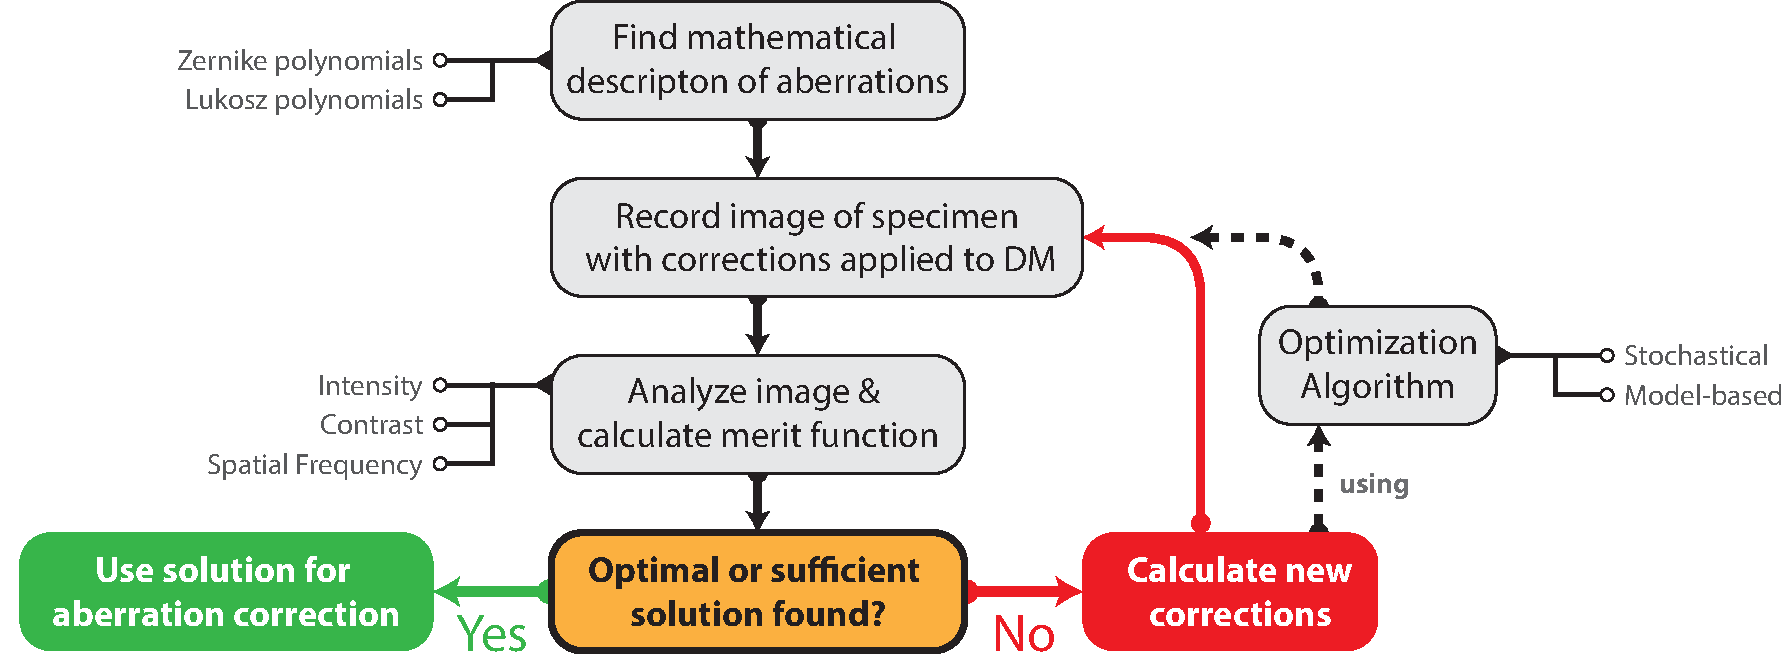
\includegraphics[width=0.75\textwidth]{images/indirect_wavefront_sensing}
	\caption{General description of the steps neccesary to perfrom indirect wavefront sensing. }
	\label{fig:indirect_wavefront_sensing}
\end{figure}


%----------------------------------------------------------------------------
\subsubsection{Stochastic Optimization}
\label{sec:GeneticAndRandomOptimizationMethods}

Several stochastic algorithms, such as hill climbing (HC), genetic (GA) and random search (RS) exist. \emph{Wright et al.}~\cite{Genetic_compared_to_others} compared these algorithms in terms of repeatability and reliability of the solutions, the final axial resolution of the system and the time taken to complete an optimization. They explain how the different algorithms can be useful, concluding that GAs have the best potential to achieve an optimal solution of the optimization process. In the context of adaptive-optical control, the genetic algorithm is well-suited because of its ability to independently optimize many variables at once~\cite{Genetic_closed_loop}. It is for that reason, that genetic algorithms are one of the most popular stochastic optimization algorithms. They try to find an optimal solution by simulating an evolution process, and the important steps are shown in Fig.~\ref{fig:genetic_algorithm_overview}. 

The basic idea of GAs is to create a population of individuals, also called chromosomes. In the case of AO, each chromosome corresponds to a specific shape of the deformable mirror. The chromosomes either represent the set of voltage applied to each actuator of the DM or, more commonly~(due to its preferable optimization performance~\cite{Genetic_smart_algorithm}), representing the set of the Zernike polynomial coefficients. After creating this initial population, each individual is evaluated and assigned a fitness value using the image quality metric. Mirror shapes, i.e. individuals, with a better fitness are closer to the optimal shape. The GA tests the entire population of individuals and selects a percentage of the most fit individuals to become parents for the next generation, called intermediate population. Then, recombination and mutation are applied to the intermediate population to create the next population. This new generation is tested again, repeating the above steps. The evolution process stops when the population includes a sufficient (or better optimal) solution. By going through this procedure, the GA gradually finds the optimal mirror shape that will yield the best solution of the quality metric. GAs do not require any preliminary information about the system but they are more time consuming than model-based approaches. Genetic algorithms are highly complex and have a large set of parameters that influence the optimization process. Those parameters are the size and randomness of initially population, the mutation and crossover rates, the size and selection of intermediate population as well as many more. A detailed description of the underlying principles and the separate steps can be found in~\cite{Genetic_tutorial} while an example where a genetic optimization algorithm is used is presented in section~\ref{sec:MultiphotonScanningMicroscopyUsingIndirektSensing}

\begin{figure}[htbp]
	\centering
		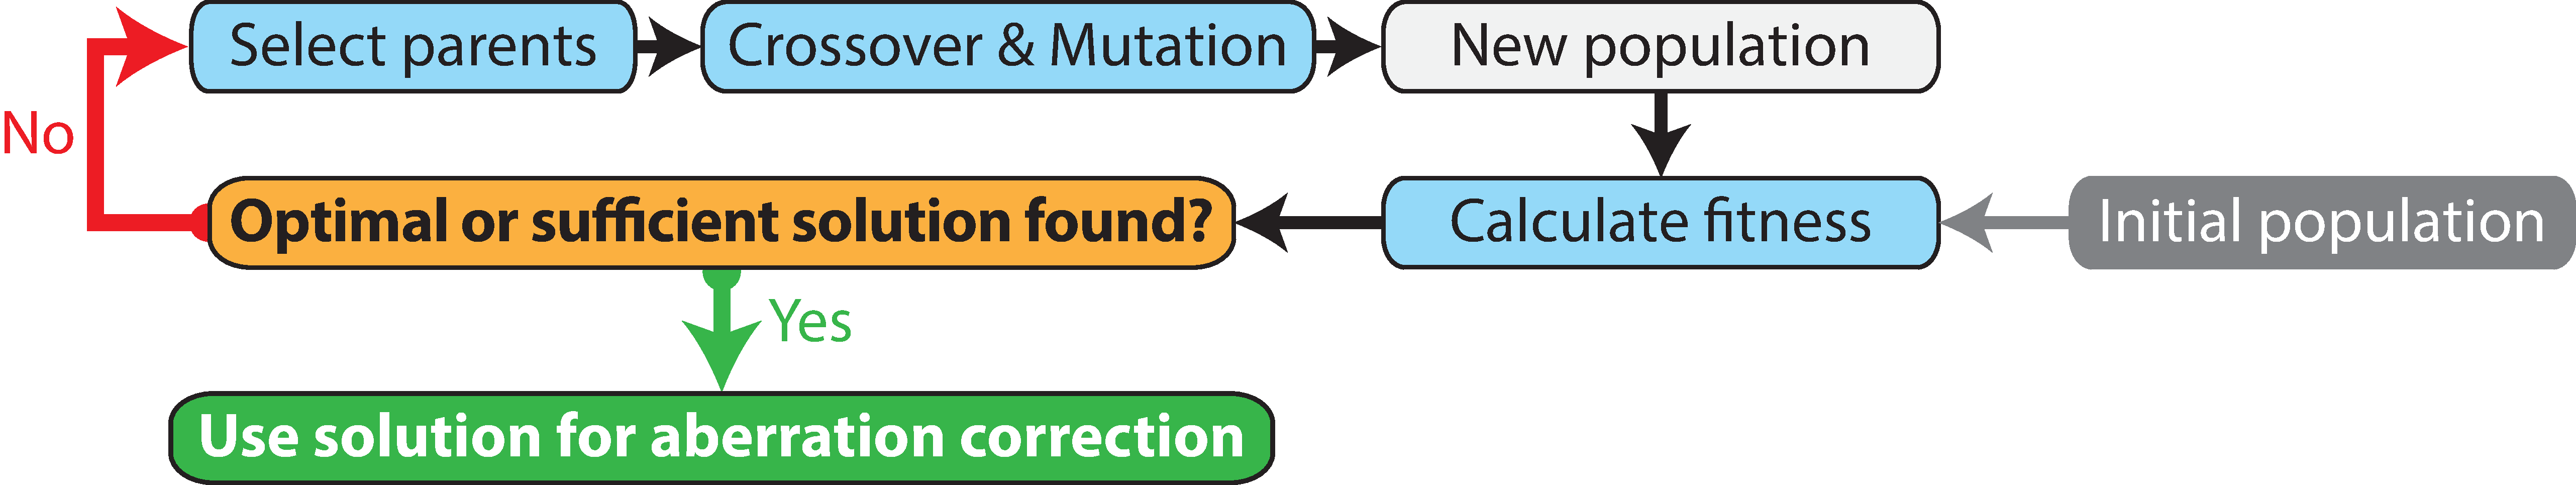
\includegraphics[width=0.70\textwidth]{images/genetic_algorithm_overview.pdf}
	\caption{Overview of a genetic algorithm. }
	\label{fig:genetic_algorithm_overview}
\end{figure}


%----------------------------------------------------------------------------
\subsubsection{Model Based Optimization}
\label{sec:ModelBasedSensing}

Methods based on a mathematical model acquire a sequence of images, each with a different, predefined aberration applied. The correction aberration is estimated from the information in this images and this process is repeated until the image quality is considered acceptable. The number of measurements needed to obtain an acceptable image depends strongly upon the optimization algorithm, the parameters used, the mathematical representation of the aberration and the object structure. For the earliest and most generic algorithms the number of measurements per aberration mode increases quadratically or exponentially with $N$, the number of corrected aberration modes~\cite{wide_sphere_packing}. The so called direct maximization method~(as described in Section~\ref{sec:TransmissionMicroscope}) is significantly more efficient, requiring only $2N+1$ measurements for $N$ modes. With this technique, Lukosz polynomials~\cite{wide_Lukosz_Modes} are used to classify the aberrations. The effects of different modes can then be separated and the optimization of each mode becomes independent and hence more efficient.

An effective model-based adaptive optics scheme should also be independent of the imaged object and should permit the separation of aberrations and object influences on the measurements. This separation is also possible through the appropriate choice of optimization metric and aberration representation~\cite{wide_AOM_loew_freq}. The interested reader will find more information on the mathematical background in reference~\cite{wide_AOM_loew_freq, wide_sphere_packing, wide_Lukosz_Modes,wide_parabolic_optimization}. 


%%%%%%%%%%%%%%%%%%%%%%%%%%%%%%%%%%%%%%%%%%%%%%%%%%%%%%%%%%%%%%%%%%%%%%%%%%%%%%%
\subsection{Aberration Correction}
\label{sec:AberrationCorrection}

The wavefront correctors are an essential part of an adaptive optics system. The goal is to apply a certain phase profile to the incident wavefront by changing either the physical length over which the wavefront propagates or the refractive index of the medium through which the wavefront goes. Wavefront correctors are build using either mirrors or liquid crystals. The former apply the phase change by adjusting their surface shape~(i.e., change their physical length while keeping the refractive index constant) while the latter keep the physical length constant and rely on localized changes in refractive index.  Mirror-based correctors are wavelength and polarization independent and can be reconfigured at rates of a few kilohertz~\cite{AOM_basic_ref}. They can have a continuous surface~(i.e., discrete actuator, bimorph or membrane mirrors) or segmented surface~(i.e. piston-only or piston/tilt mirrors) as shown in Fig.~\ref{fig:Correctors}. Unlike continuous mirrors, the segmented mirrors have gaps between the segments that reduce the efficiency and quality of the correction, although they can achieve much better wavefront fitting. 

\begin{figure}[tbh]
			\centering
			\begin{subfigure}[b]{0.25\textwidth}
							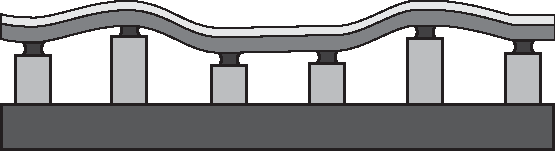
\includegraphics[width=\textwidth]{images/deformable_discrete}
							\caption{Discrete}
							\label{fig:Correctors_discrete}
			\end{subfigure}
			\quad
			\begin{subfigure}[b]{0.25\textwidth}
							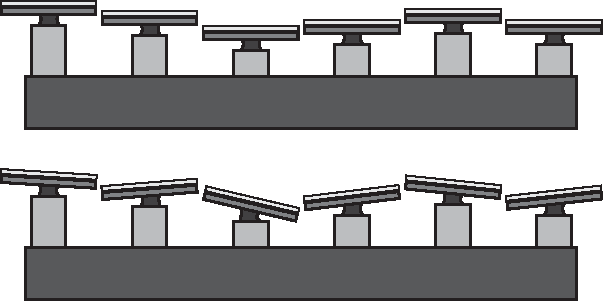
\includegraphics[width=\textwidth]{images/deformable_piston}
							\caption{Piston-Only}
							\label{fig:Correctors_piston}
			\end{subfigure}
			
			\vspace{5mm}
			
			\begin{subfigure}[b]{0.25\textwidth}
							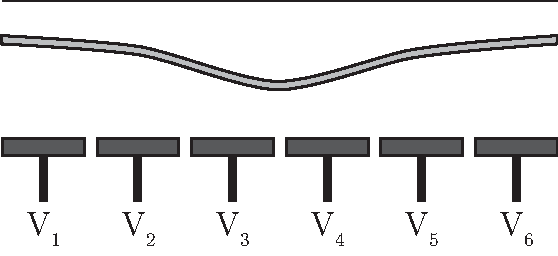
\includegraphics[width=\textwidth]{images/deformable_membrane}
							\caption{Membrane}
							\label{fig:Correctors_membrane}
			\end{subfigure}
			\quad
			\begin{subfigure}[b]{0.25\textwidth}
							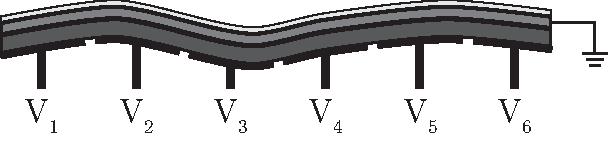
\includegraphics[width=\textwidth]{images/deformable_bimorph}
							\caption{Bimorph}
							\label{fig:Correctors_bimorph}
			\end{subfigure}							
			\caption{The four main mirror correctors. (a) Discrete actuator deformable mirrors consist of a continuous, reflective surface and an array of actuators, each capable of producing a local deformation in the surface. (b) Piston-only segmented correctors consist of an array of small planar mirrors whose axial motion~(piston) is independently controlled. Piston/tip/tilt-segmented correctors add independent tip and tilt motion to the piston-only correctors. (c) Membrane mirrors and (d) Bimorph mirrors. Image after~~\cite{AO_vision_science}.}
	\label{fig:Correctors}
\end{figure} 


Liquid crystal-based modulators change the refractive index electronically or optically, are wavelength and polarization dependent and can reach velocities of just a few tens of hertz. The nematic liquid crystal is the most common for AO applications. In general, they are much cheaper than the mirror-based correctors, are capable of producing more complex phase patterns but they have lower light efficiency due to absorption.   

In AO microscopes the first choice in most cases is the deformable mirror because of the higher light efficiency and velocity. Furthermore, they are better suited for fluorescence techniques due to their polarization independent behavior. However, in particular cases, liquid-crystal modulators can be sufficient if aberration correction is only needed in the illumination path.
